\section{Results/Discussion}
Performance results varied across the board between the three language implementations. Table 1 quantifies the time reduction factor observed in untyped languages relative to their typed counterparts. For example, arithmetic operations in Cython take only 0.1964x of the execution time required for their Python counterparts. The compiled languages of Cython and TypeScript have the most obvious performance benefits with a geometric mean time reduction of 0.3570 and 0.8363 respectively. Hack has a surprising increase of 1.0006 which suggests that adding type annotations to this test suite does little to improve its performance and may even be detrimental. 

\begin{table}[H]
\centering
\begin{tabular}{llll}
           & Python            & PHP               & Javascript        \\
arithmetic & 0.196480938416422 & 1.08117249154453  & 0.521531100478469 \\
strings    & 0.417322834645669 & 1                 & 0.994459833795014 \\
io         & 0.943697216140131 & 0.946666666666667 & 0.934271370062095 \\
recursion  & 0.210092414068214 & 0.979452054794521 & 1.0098452883263  
\end{tabular}
\caption{Time reduction factor for untyped implementation vs typed. Values \textgreater 1 imply that typed implementations are slower. Values \textless 1 imply that typed implementations are faster.}\label{tab:slowdownfactor}
\end{table}

\subsection{PHP/HACK}
Adams et al. \cite{Adams:2014:HVM:2660193.2660199} have determined that HHVM performance can achieve a geometric mean speedup of 2.64x within their internal benchmark suites. Results in this paper do not agree with the benchmarks of Adams et al. Figure \ref{fig:phpHackRaw} depicts the runtime (in seconds) of PHP and Hack versions. Figure \ref{fig:phpHackRelative} depicts the relative runtime where blue represents Hack and red represents PHP. Only the IO and recursive benchmarks in Hack provide a runtime advantage over PHP, and even these are within the margin of error for this experiment. Usage of Hack and HHVM do not provide any tangible benefit to performance with this test suite. It is likely that these benchmarks do not cover enough features that expose the performance of the HHVM Jit. However, the benefit of utilizing HHVM in strict mode is that it is type sound, and developers can be confident that type errors will not be encountered during runtime. 

\begin{figure}[H]
\centering
\begin{subfigure}{.5\textwidth}
  \centering
  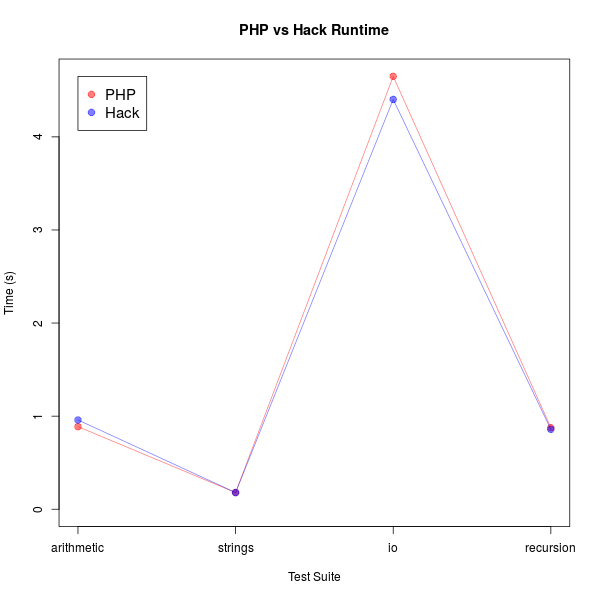
\includegraphics[width=\linewidth]{../src/PHP_typed_vs_untyped.png}
  \caption{PHP Typed vs Untyped Runtime}
  \label{fig:phpHackRaw}
\end{subfigure}%
\begin{subfigure}{.5\textwidth}
  \centering
  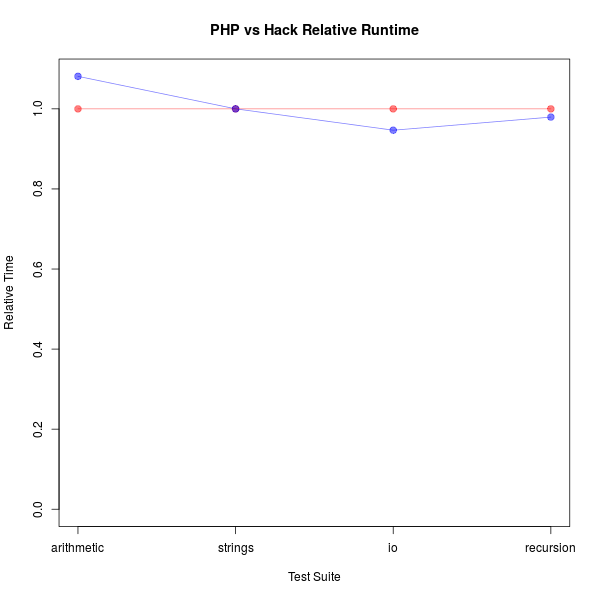
\includegraphics[width=\linewidth]{../src/PHP_typed_vs_untyped_relative.png}
  \caption{PHP vs Hack Runtime Reduction}
  \label{fig:phpHackRelative}
\end{subfigure}
\caption{\ref{fig:phpHackRaw}: Depicts runtime in seconds. \ref{fig:phpHackRelative}: Depicts relative runtime. Blue refers to Hack and is scaled to 1x runtime reduction. Red values refer to PHP. Lower values are better.}
\label{fig:phpHack}
\end{figure}


\subsection{Python/Cython}
From the literature review on related work in Section \ref{Related Work}, it was observed that Cython implementations can accelerate Python programs by compiling them to C code. Speedups of approximately 30x were observed in a function that implements mathematical operations such as addition, division, iterations over a loop, and multiplication. Results observed in this paper support this claim, however the speedup factor is not as extreme as observed by Wilbers et al. It is clear from Figure \ref{fig:pythonCythonRaw} that Cython arithmetic, string and recursive functions are all notably faster than their Python counterparts, indicated by their lower runtime (in seconds) whereas IO operations are relatively similar but still faster. Figure \ref{fig:pythonCythonRelative} depicts the relative runtime where blue represents Cython and red represents Python. 

\begin{figure}[H]
\centering
\begin{subfigure}{.5\textwidth}
  \centering
  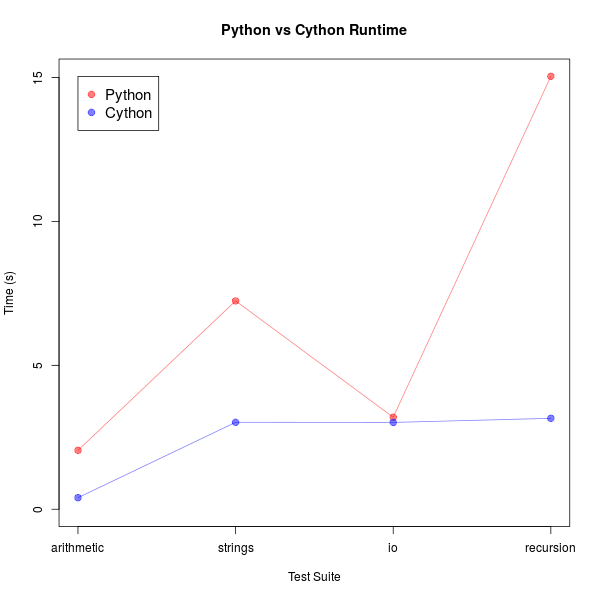
\includegraphics[width=\linewidth]{../src/Python_typed_vs_untyped.png}
  \caption{Python vs Cython Runtime}
  \label{fig:pythonCythonRaw}
\end{subfigure}%
\begin{subfigure}{.5\textwidth}
  \centering
  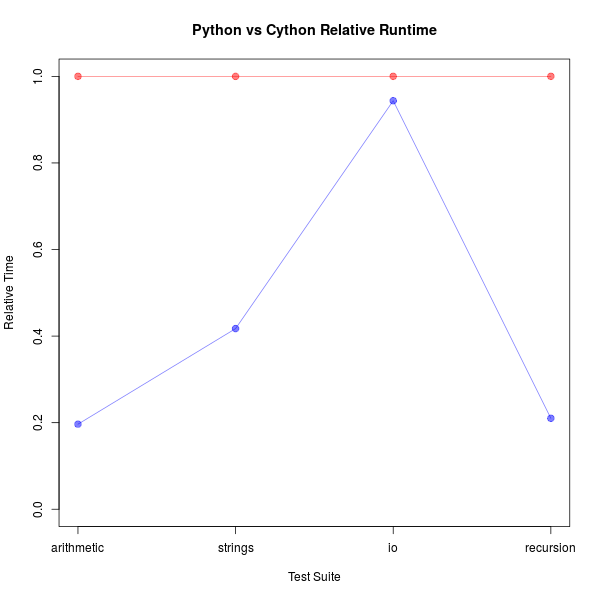
\includegraphics[width=\linewidth]{../src/Python_typed_vs_untyped_relative.png}
  \caption{Python vs Cython Runtime Reduction}
  \label{fig:pythonCythonRelative}
\end{subfigure}
\caption{\ref{fig:pythonCythonRaw}: Depicts runtime in seconds. \ref{fig:pythonCythonRelative}: Depicts relative runtime. Blue refers to Cython  and is scaled to 1x runtime reduction. Red values refer to Python. Lower values are better.}
\label{fig:pythonCython}
\end{figure}



\subsection{JavaScript/TypeScript}

\begin{figure}[H]
\centering
\begin{subfigure}{.5\textwidth}
  \centering
  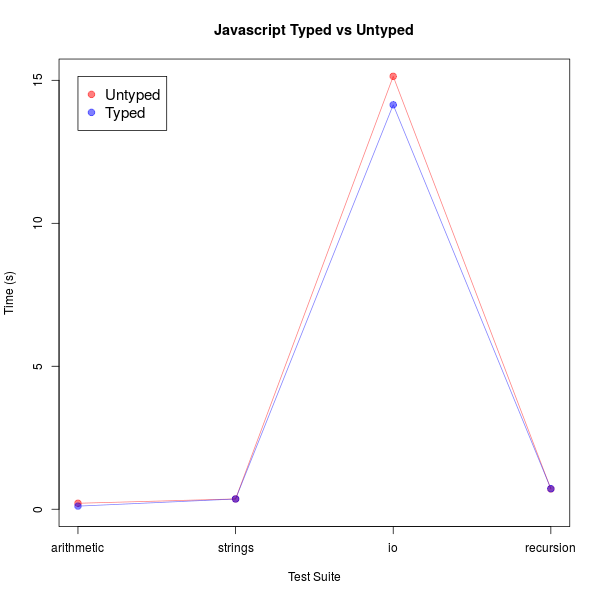
\includegraphics[width=\linewidth]{../src/Javascript_typed_vs_untyped.png}
  \caption{JavaScript vs TypeScript Runtime}
  \label{fig:javascriptTypescriptRaw}
\end{subfigure}%
\begin{subfigure}{.5\textwidth}
  \centering
  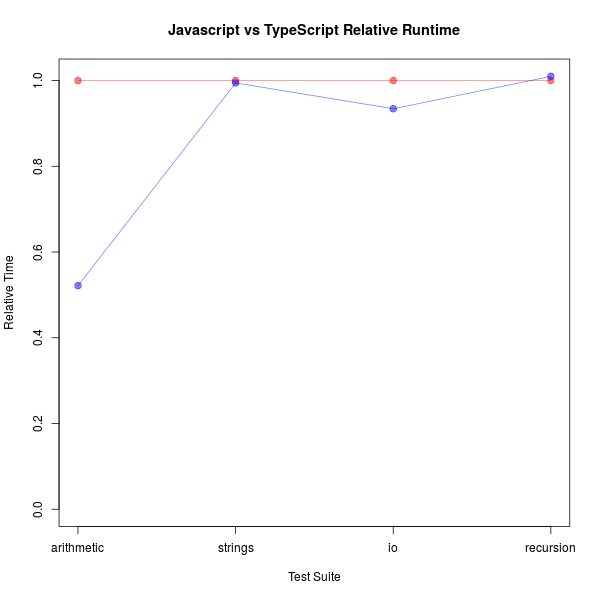
\includegraphics[width=\linewidth]{../src/Javascript_typed_vs_untyped_relative.png}
  \caption{JavaScript vs TypeScript Runtime Reduction}
  \label{fig:javascriptTypescriptRelative}
\end{subfigure}
\caption{\ref{fig:javascriptTypescriptRaw}: Depicts runtime in seconds. \ref{fig:javascriptTypescriptRelative}: Depicts relative runtime. Blue refers to TypeScript  and is scaled to 1x runtime reduction. Red values refer to JavaScript. Lower values are better.}
\label{fig:javascriptTypescript}
\end{figure}


\subsection{Threats To Validity}
The primary threat to validity for this project is that the benchmarks are nowhere near comprehensive enough to encapsulate all potential use cases of each language. Results generated by this work may not be generalizable to other programming languages, or even the languages examined by this paper. This lack of generalizability is evidenced by the lack of agreement between this paper's results on HHVM and other work on JIT-compiled PHP.
Another threat to validity could be that these tests are not representative of the actual runtime of functions, as functions are called an arbitrary number of times in order to generate numbers for plotting. A more sensible approach would be to incrementally increase the amount of iterations that each function is called. This would have the effect of identifying any side effects of the iteration process. Additionally, a more precise benchmarking tool could be used to measure runtimes as this would eliminate the need to iteratively call functions altogether.


\subsection{Future Work}
Much of the initial effort of this work went into configuring the environment within the docker container in order to properly compile and run each language. Benchmarks implemented in this paper are very rudimentary and would be improved upon by adding code that implements inheritance relationships, complex data structures and callbacks or anonymous functions. Additionally, more complex benchmarking tools that examine characteristics such as memory usage, CPU statistics and even stack traces would be more beneficial and informative for individuals interested in researching the costs of type safety. Different configurations of the docker container could be set up in order to mimic memory swapping in a production environments. 


